\documentclass{jsbook}
\setlength{\textwidth}{\fullwidth}
\setlength{\evensidemargin}{\oddsidemargin}
\usepackage{color}
\usepackage{amsmath}
\usepackage[dvipdfmx]{graphicx}
\begin{document}
1.1時間積分

 1.1.1 leap frogによる時間積分と時間フィルター(10月日本語済 1月英訳予定)

1.2 トレーサー移流スキーム (11月日本語済 添削待ち 12月修正・不足箇所追加+ハイブリッド座標について追加)

1.3力学部分まとめ

 1.3.1 時間フィルター (10月日本語済 1月英訳予定)
\chapter{力学過程}
\section{時間積分}
時間差分スキームは基本的にleap frogである。

ただし、拡散項および物理過程の項は後方差分もしくは前方差分とする。計算モードを抑えるために時間フィルター(Williams, 2009)を用いる。

さらに$\Delta t$を大きくとるために、重力波の項にsemi-impicitの手法を適用する(Bourke,1988)。
\subsection{leap frogによる時間積分と時間フィルター}
leap frogにおける計算モードの影響緩和のためにWilliams(2009)の時間フィルターを毎ステップごとに適用する。

時間フィルターは以下の式で与えられる。

バーは時間フィルターがかかっていることを意味する。
\begin{equation}   
\bar{\bar{X}}^{t} = \bar{X}^{t} + \nu \alpha [\bar{\bar{X}}^{t-\Delta t} - \bar{X}^{t} + X^{t+\Delta t}] 
\end{equation}
\begin{equation}   
\bar{X}^{t+\Delta t} = X^{t+\Delta t} + \nu (1-\alpha) [\bar{\bar{X}}^{t-\Delta t} - 2 \bar{X}^{t} + X^{t+\Delta t}] 
\end{equation}
ただし、$\nu=0.05$かつ、$\alpha=0.5$である。
\section{トレーサー移流スキーム}
\subsection{スペクトル法の限界と移流スキームの導入}
MIROC6は力学フレームとして球面調和関数展開に基づくスペクトル法を採用しているのはこれまで述べてきたとおりである。

スペクトル法の欠点として例えば以下のようなものがある。
\begin{enumerate}
\item Gibbs現象のため、滑らかでない分布を表現しようするとノイズ的な振動が出てしまう。
\item 上の現象と関連し、本来物質量としてはありえない負の値が変換格子点上に出現する。
\item グローバルな保存性は良いが、ローカルに見ると必ずしも保存性を満たさない。
\item 情報が上流から下流のみにローカルに伝わるという性質(移流性)が必ずしも満たされない(極端にいえば、地球の裏側まで情報が瞬時に伝わる)。
\end{enumerate}
以上の短所を了承した上でMIROCでは力学の基本フレームとしてスペクトル法を採用している。

Gibbs現象による短所も大抵の場合深刻な問題は生じない。

しかし、特に不連続性の強い分布をもつ物質の輸送に関しては、場合によってはノイズや負の値が相対的に目立ち、看過できない場合が生じる。

例えば、極や成層圏など水蒸気の分布は不連続になりやすく、エアロゾルなどもともと局所集中的な分布を持ちがちな変数の輸送にはGibbs現象の影響は現れやすい(水蒸気の輸送は補正を行うことで影響を緩和することができる)。

そこで、MIROC6では水蒸気輸送とトレーサーの輸送に関してはスペクトル法を用いず、Lin and Rood(1996)のフラックス形式semi-Lagrange(FFSL)スキームを用いて計算している。このスキームは以下の利点がある
\begin{enumerate}
\item 格子点法を基本とするためGibbs現象が生じず、滑らか出ない場を精度良く表現できる。
\item 上流から下流への移流性を満たす。
\item ローカルおよびグローバルな保存性を満たす。
\item 極で格子間隔が狭くなることによる問題が回避できる。
\end{enumerate}
ここではMIROC6で採用いているトレーサー移流スキームについて記述する。

\subsection{MIROC6のトレーサー移流スキームの概要}
\subsubsection{フラックス形式の輸送方程式}
例として$x,y,p$直交座標系における3次元移流方程式を考えると以下のようになる。

\begin{equation}
\frac{\partial q}{\partial t} = -u \frac{\partial q}{\partial x}-v \frac{\partial q}{\partial y}-\omega \frac{\partial q}{\partial p}
\end{equation}
これと連続の式を組み合わせると、フラックス形式の輸送方程式
\begin{equation}
  \frac{\partial q}{\partial t}=-\frac{\partial}{\partial x}(uq)-\frac{\partial}{\partial y}(vq)-\frac{\partial}{\partial p}(\omega q)
  =-\frac{\partial}{\partial x}F^{x}-\frac{\partial}{\partial y}F^{y}-\frac{\partial}{\partial p}F^{p}
\end{equation}
を得る。

$x=x_{i} (i=1,2,3...), y=y_{j} (j=1,2,3...), p=p_{k} (k=1,2,3...)$で格子点法で離散化すると
\begin{equation}
  \frac{\partial q_{i,j,k}}{\partial t}=\frac{1}{\Delta x_{i,j,k}}(F^{x}_{i-\frac{1}{2},j,k}-F^{x}_{i+\frac{1}{2},j,k})+\frac{1}{\Delta y_{i,j,k}}(F^{y}_{i,j-\frac{1}{2},k}-F^{y}_{i,j+\frac{1}{2},k})+\frac{1}{\Delta p_{i,j,k}}(F^{p}_{i,j,k-\frac{1}{2}}-F^{p}_{i,j,k+\frac{1}{2}})
\end{equation}
ここで、$F^{x}_{i-\frac{1}{2},j,k}$は格子$(i,j,k)$と格子$(i-1,j,k)$の境界における$x$方向のフラックス、$\Delta x_{i,j,k}$は格子$(i,j,k)$の代表する$x$方向の幅である。

このようなフラックス形式を基本とすると、保存性は自動的に満たされる。

スキームの精度等は$F^{x}_{i-\frac{1}{2},j,k}$等の選択に依存する。

次でMIROC6で採用されている$F^{x}_{i-\frac{1}{2},j,k}$の選択法を簡単のために$x$方向1次元で説明する。
\subsubsection{The Piecewise Parobolic Method (PPM) スキーム}
semi-Lagrangeスキームでは時刻tにおける地点$x_{i+\frac{1}{2}}$のフラックスを計算するのに時刻$t-\Delta t$の地点$x_{i+\frac{1}{2}}-u\Delta t$の$q$の値を用いる。$u$には時刻$t$の値、$q$には時刻$t-\Delta t$の値を用いることになる。

CFL条件($|\frac{u\Delta t}{\Delta x}|<1$)を満たし、$u_{i+\frac{1}{2}}>0$の場合$x_{i+\frac{1}{2}}-u\Delta t$はグリッド$i$の内部の地点になる。

地点$x_{i+\frac{1}{2}}-u\Delta t$の$q$の値としてはグリッド$i$内では$q$が一定値をとるとしてグリッド$i$での平均値$q_{i}$を選ぶ方法もある。

しかし、これはグリッド$i$と$i+1$の境界$i+\frac{1}{2}$で$q$の大きな不連続があることになり、数値粘性が強くなってしまって数値計算的に望ましくない。

そこでグリッド内で一定値としていた$q$の値に何らかの分布を与えて、境界$i+\frac{1}{2}$での不連続を無くし、$x_{i+\frac{1}{2}}-u\Delta t$の地点の$q$の値を内挿から求める事ができるようにしたい。

与えられた分布は以下を満たさなければならない。

\begin{equation}
  q_{i}=\frac{1}{\Delta x_{i}} \int_{x_{i+\frac{1}{2}}}^{i-\frac{1}{2}} q(x) dx
\end{equation}

旧版のMIROCでは1次関数を内挿するVan Leer法が用いられていたが、現行のMIROCでは3次関数で内挿するThe Piecewise Parobolic Method (PPM)スキーム(Colella and Woodward 1984)が用いられている(図\ref{f1})。

\begin{figure}
  \centering
  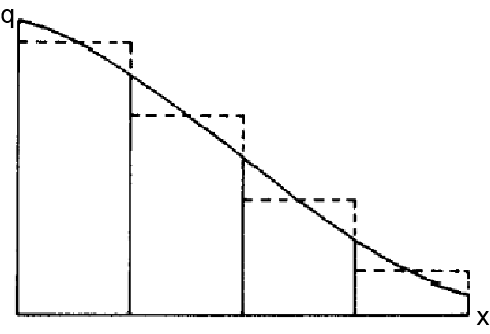
\includegraphics[width=5cm]{ppm_interpolate.png}
  \caption{PPMスキームの内挿のイメージ。点線はグリッド平均値。実線は内挿関数}
    \label{f1}
\end{figure}
ここからPPMスキームによる内挿を見ていく。

PPMでは以下のように$q$の分布を定める。
\begin{equation}
\begin{split}
\label{a4}
  q(x)=q_{L,i}+\xi (\Delta q_{i}+q_{R,i}(1-\xi))\\
  \xi=\frac{x-x_{i-\frac{1}{2}}}{\Delta x_{i}},  x_{i-\frac{1}{2}}\leq x \leq x_{i+\frac{1}{2}}
  \end{split}
\end{equation}
ここで、$q_{L,i}$は$\lim_{x \to x_{i+\frac{1}{2}}}=q_{L,i}$と定義される。

同様に$q_{R,i}$も$\lim_{x \to x_{i+\frac{1}{2}}}=q_{R,i}$と定義される。

この内挿では境界$i+\frac{1}{2}$では$q$は連続なので、$q_{L,i+1}=q_{R,i}=q_{i+\frac{1}{2}}$となる。

また、
\begin{equation}
  \Delta q_{i}=q_{R,i}-q_{L,i},\qquad q_{6,i}=6(q_{i}-\frac{1}{2}(q_{L,i})+q_{R,i})
\end{equation}
である。

$q_{i+\frac{1}{2}}$を内挿するにあたり、以下のような$a$の有限積分を考える。
\begin{equation}
  A(x)= \int^{x} q(x') dx'
\end{equation}
グリッドの境界では
\begin{equation}
A(x_{i+\frac{1}{2}})=A_{i+\frac{1}{2}}=\sum_{k\leq i}q_{k}\Delta x_{k}  
\end{equation}
となる。

$q_{i+\frac{1}{2}}$は$(A_{j+k+\frac{1}{2}},x_{j+k+\frac{1}{2}})$, $k=0,\pm 1, \pm 2$を用いて$q_{i+\frac{1}{2}}=dA/dx |_{x_{i+\frac{1}{2}}}$を離散化することで求めて

\begin{equation}
  \label{a3}
  \begin{split}
    q_{i+\frac{1}{2}}=&q_{i}+\Delta x_{i} \frac{q_{i+1}-q_{i}}{\Delta x_{i+1}+\Delta x_{i}}+\frac{1}{\sum_{k=i-1}^{i+2}\Delta x_{k}}\\
    &\times \Bigl[\frac{2\Delta x_{i}\Delta x_{i+1}}{\Delta x_{i+1}+\Delta x_{i}}(\frac{\Delta x_{i}+\Delta x_{i-1}}{\Delta x_{i+1}+2\Delta x_{i}}-\frac{\Delta x_{i+2}+\Delta x_{i+1}}{2\Delta x_{i+1}+\Delta x_{i}})(q_{i+1}-q_{i})\\
     & -\Delta x_{i}\frac{\Delta x_{i}+\Delta x_{i-1}}{\Delta x_{i+1}+2\Delta x_{i}} \delta q_{i+1}+\Delta x_{i+1} \frac{\Delta x_{i+2}+\Delta x_{i+1}}{2\Delta x_{i+1}+\Delta x_{i}} \delta q_{i}\Bigr]
  \end{split}
\end{equation}
となる。

ただし、グリッド幅が等間隔の場合(東西方向を計算する際に適用)には式(\ref{a3})は簡略化されて

\begin{equation}
  q_{i+\frac{1}{2}}=\frac{1}{2}(q_{i-1}+q{i})-\frac{1}{6}(\delta q_{i}-\delta q_{i-1})
\end{equation}
と表せる。

ここで$\delta q_{i}$は
\begin{equation}
  \delta q_{i}=\frac{\Delta x_{i}}{\Delta x_{i-1}+\Delta x_{i}+\Delta x_{i+1}}\biggl[\frac{2\Delta x_{i-1}+\Delta x_{i}}{\Delta x_{i+1}+\Delta x_{i}}(q_{i+1}-q_{i})+\frac{\Delta x_{i}+2\Delta x_{i+1}}{\Delta x_{i-1}+\Delta x_{i}}(q_{i}-q_{i-1})\biggr]
\end{equation}
と与えられる。

しかし、これでは内挿した関数がグリッド内で極値を持つ場合などは単調性が保てない場合があるので、$q_{i+\frac{1}{2}}$が$q_{i}$と$q_{i+1}$の間にあるように$\delta q_{i}$を
\begin{equation}
  \begin{aligned}
    \delta_{m} q_{i} & =\min(|\delta
    q_{i}|,2|q_{i}-q_{i-1}|,|q_{i+1}-q_{i}|) && \qquad \text{if$\quad(q_{i+1}-q_{i})(q_{i}-q_{i-1}) >0$}, \\
    & =0 && \qquad \text{otherwise}
  \end{aligned}
\end{equation}
と改良し、これを$\delta q_{i}$として式(\ref{a3})に用いて$q_{i+\frac{1}{2}}$を求める。

(\ref{a4})式のように$q(x)$が内挿されるとき、CFL数を以下のように定義すると
\begin{equation}
  C=\frac{u_{i+\frac{1}{2}}\Delta t}{\Delta x_{i+1}}
\end{equation}
フラックス$F^{x}_{i+\frac{1}{2}}$は
\begin{equation}
  F^{x}_{i+\frac{1}{2}}=\begin{cases}u_{i+\frac{1}{2}}[q_{R,i}-\frac{C}{2}(\Delta q_{i}-(1-\frac{2}{3}C)q_{6,i})] & (u_{i+\frac{1}{2}}\ge0)\\
  u_{i+\frac{1}{2}}[q_{L,i+1}+\frac{C}{2}(\Delta q_{i+1}+(1-\frac{2}{3}C)q_{6,i+1})] & (u_{i+\frac{1}{2}}\leq0)
  \end{cases}
\end{equation}
\subsubsection{長い時間ステップをとるための工夫}
以上の議論はCFL数Cの絶対値が1以下の場合のみ安定である。

格子法を球面上に適用する場合、極付近では$\Delta x$が小さくなるため、かなり小さな$\Delta t$を用いない限り、そのまま適用できない。

この問題を回避し、$\Delta t$を大きくとるための工夫として、Cの絶対値が1を超える場合は以下のように扱う。

この方法は一般の格子間隔の場合も利用できるが、以下では$\Delta x$がiに依存しないとして記述する。

CFL数を
\begin{equation}
  C=I_{C}+\hat{C},\quad I_{C}:整数,\quad -0.5\le \hat{C} \le 0.5
\end{equation}
のように整数部$I_{C}$と小数部$\hat{C}$に分ける。

$I_{C}>0$のとき、
\begin{equation}
  F^{x}_{i-\frac{1}{2}}=\hat{F^{x}_{i-I_{C}+\frac{1}{2}}}+\sum^{i}_{i'=i+1-I_{C}} q_{i'} \frac{\Delta x_{i}}{\Delta t}
\end{equation}
$I_{C}<0$のとき、
\begin{equation}
  F^{x}_{i-\frac{1}{2}}=\hat{F^{x}_{i+|I_{C}|+\frac{1}{2}}}+\sum^{i+|I_{C}|}_{i'=i+1} q_{i'} \frac{\Delta x_{i}}{\Delta t}
\end{equation}
ただし、$\hat{F^{x}_{i-I_{C}+\frac{1}{2}}}$は、格子$(i-I_{C}+\frac{1}{2})$においてCFL数の小数部$\hat{C}$を用いて計算したフラックスである。

  このように、$\Delta t$の間に複数格子分流体が移動する場合も、通過するそれぞれの格子に対応した物理量$q_{i'}$を用いてフラックスを評価することにより、物理的に整合的になり、計算の不安定を避けられる。

  以上の手続きはCFL条件を破る可能性がある東西方向の計算にのみ適用される。

  \subsubsection{クロス・タームの考慮}
  流れが純粋に$x$方向あるいはy方向ではなく、$u、v$ともに0でない場合、$C$が比較的大きいと、$x$方向、$y$方向のフラックスの寄与をただ足し合わせただけでは、斜め方向への移流の効果が過小評価となる。

  そこで、このようなクロス・タームを考慮するため、以下のような手続きを行う。

  ここでは1次元ではなく、2次元空間で議論を行う。
  
  $x$方向のフラックス$F^{x}_{i+\frac{1}{2},j}$の計算に使用する際の$q$の値として、格子点$q_{i,j}$の代わりに、semi-Lagrange法の考え方を導入した$y$方向の上流側の平均値
  \begin{equation}
    q^{y}_{i,j}=\frac{1}{2} {q(x_{i},y_{i}-v_{i,j}\Delta t)+q_{i,j}}
  \end{equation}
  を用いる。ここで、$q(x_{i},y_{i}-v_{i,j}\Delta t)$は、近傍の点からの補間(最近接の2点の線形補間)によって求める。

  同様に$y$方向のフラックス$F^{y}_{i,j+\frac{1}{2}}$の計算に使用する際の$q$の値としては、x方向の上流側の平均値
  \begin{equation}
    q^{x}_{i,j}=\frac{1}{2} {q(x_{i}-u_{i,j}\Delta t,y_{i})+q_{i,j}}
  \end{equation}
  を用いる。
  3次元輸送の場合は、この補間を2次元で行う。

  
  \subsection{実際の移流スキームの手順($\sigma$座標系)}
球面上の$\sigma$座標での輸送方程式は
\begin{eqnarray}
  \label{b1}
  \frac{\partial P^{s} q}{\partial t} &=& - \frac{1}{a \cos \varphi} \frac{\partial}{\partial \lambda}(P^{s} uq)- \frac{1}{a \cos \varphi} \frac{\partial}{\partial \varphi}(P^{s} vq \cos \varphi)- \frac{\partial}{\partial \sigma} (P^{s} \dot{\sigma} q)\\
  &=& \frac{1}{a \cos \varphi} \frac{\partial}{\partial \lambda}(F^{\lambda})- \frac{1}{a \cos \varphi} \frac{\partial}{\partial \varphi}(F^{\varphi})- \frac{\partial}{\partial \sigma} (F^{\sigma})
\end{eqnarray}
$P^{s}$は地表面気圧、$q$はトレーサーの量である(ex. 混合比for水蒸気量)。

連続の式は$q=1$の時を考えて
\begin{equation}
  \frac{\partial P^{s}}{\partial t} = - \frac{1}{a \cos \varphi} \frac{\partial}{\partial \lambda}(P^{s}u)- \frac{1}{a \cos \varphi} \frac{\partial}{\partial \varphi}(P^{s}v \cos \varphi)- \frac{\partial}{\partial \sigma} (P^{s} \dot{\sigma})
\end{equation}
ここで、格子は軽度方向に等間隔として離散化を考えると輸送方程式は
\begin{equation}
\label{a1}
  \frac{\partial P^{s}_{,i,j,k} q_{i,j,k}}{\partial t}=\frac{1}{\Delta D_{j,k}}[(G^{\lambda}_{i-\frac{1}{2},j,k}-G^{\lambda}_{i+\frac{1}{2},j,k})+(G^{\varphi}_{i,j-\frac{1}{2},k}-G^{\varphi}_{i,j+\frac{1}{2},k}))+(G^{\sigma}_{i,j,k-\frac{1}{2}}-G^{\sigma}_{i,j,k+\frac{1}{2}})]
\end{equation}
と表される。ただし、
\begin{equation}
  G^{\lambda}_{i-\frac{1}{2},j,k}=F^{\lambda}_{i-\frac{1}{2},j,k} \Delta y_{j} \Delta \sigma_{k}=(P^{s}uq)_{i-\frac{1}{2},j,k} \Delta y_{j} \Delta \sigma_{k}
\end{equation}
\begin{equation}
  G^{\varphi}_{i,j-\frac{1}{2},k}=F^{\varphi}_{i,j-\frac{1}{2},k} \Delta x_{j-\frac{1}{2}} \Delta \sigma_{k}=(P^{s}vq)_{i,j-\frac{1}{2},k} \Delta x_{j-\frac{1}{2}} \Delta \sigma_{k}
\end{equation}
\begin{equation}
  G^{\sigma}_{i,j,k-\frac{1}{2}}=F^{\eta}_{i,j,k-\frac{1}{2}} \Delta x_{j} \Delta y_{j}=(P^{s} \dot{\sigma} q)_{i,j,k-\frac{1}{2}} \Delta x_{j} \Delta y_{j}
\end{equation}
また、
\begin{equation}
  \Delta D_{j,k}=a \cos \varphi_{j} \Delta \lambda \Delta \varphi_{j} \Delta \sigma_{k},\quad \Delta x_{j}=a \cos \varphi_{j} \Delta \lambda,\quad \Delta y_{j}=a \Delta \varphi_{j}
\end{equation}
である。このようなフラックス形式を基本とすると、保存性は自動的に満たされる。

精度及び単調性を満たすか否かは$F^{\lambda}_{i-\frac{1}{2},j,k}$の決定法などに依存する。

ここからは離散化された移流方程式を実際にはどのように解いているのかを見ていく。

スペクトルモデルでは、変換格子$(i,j,k)$上の同じ点(整数点)で、u,vおよびスカラー量が計算される。

スペクトル逆変換を用いれば、格子の境界における$u,v$の値、すなわち$u_{i-\frac{1}{2},j,k},v_{i,j-\frac{1}{2},k}$を求める事が可能であるが、そのようにして求めた$u_{i-\frac{1}{2},j,k},v_{i,j-\frac{1}{2},k}$は必ずしも連続の式の差分系を満たさない。

連続の式の差分系は離散化された移流方程式で$q=1$の時を考えて
\begin{equation}
  \frac{\partial P^{s}_{i,j,k} }{\partial t}=\frac{1}{\Delta D_{j,k}}[(V^{\lambda}_{i-\frac{1}{2},j,k}-V^{\lambda}_{i+\frac{1}{2},j,k})+(V^{\varphi}_{i,j-\frac{1}{2},k}-V^{\varphi}_{i,j+\frac{1}{2},k}))+(V^{\sigma}_{i,j,k-\frac{1}{2}}-V^{\sigma}_{i,j,k+\frac{1}{2}})]
\end{equation}
で与えられる。ただし、
\begin{equation}
  V^{\lambda}_{i-\frac{1}{2},j,k}=(P^{s}u)_{i-\frac{1}{2},j,k} \Delta y_{j} \Delta \sigma_{k}
\end{equation}
\begin{equation}
  V^{\varphi}_{i,j-\frac{1}{2},k}=(P^{s}v)_{i,j-\frac{1}{2},k} \Delta x_{j-\frac{1}{2}} \Delta \eta_{k}
\end{equation}
\begin{equation}
  V^{\sigma}_{i,j,k-\frac{1}{2}}=(P^{s}\dot{\sigma})_{i,j,k-\frac{1}{2}} \Delta x_{j} \Delta y_{j}
\end{equation}
以上の課題はスペクトルモデルの水平質量収束の場から、この格子系で離散化された連続の式を満たすように水平・鉛直流を再構成することによって(ほぼ)この問題を解決する。

MIROC6におけるトレーサー移流スキームの具体的な計算手順は以下のとおりである。
\begin{enumerate}
\item スペクトル法で、トレーサー量($q$)以外の量($P^{s}(t+\Delta t), \bf{v}(t+\Delta t)$)を予報する。
\item 球面調和関数展開により、連続の方程式の右辺第1項$C^{x}_{i,j,k}$および第2項$C^{y}_{i,j,k}$を評価する。
  \begin{equation}
    C^{x}=-\frac{1}{a \cos \varphi}\frac{\partial}{\partial \lambda}(P^{s}u),\quad C^{y}=-\frac{1}{a \cos \varphi}\frac{\partial}{\partial \lambda}(P^{s}v \cos \varphi) 
  \end{equation}
  このとき、$(t-\Delta t)$と$(t+\Delta t)$の平均の風の場を用いる。これは$P^{s}$の時間積分にsemi-implicitを用いているからである。
\item $C_{x}$,$C_{y}$を用い、$V^{\lambda}, V^{\varphi}, V^{\sigma}$を求める。
  \begin{equation}
    V^{\lambda}_{i-\frac{1}{2},j,k}-V^{\lambda}_{i+\frac{1}{2},j,k}=C^{x}_{i,j,k}\Delta D_{j,k}, \quad V^{\lambda}_{i,j-\frac{1}{2},k}-V^{\lambda}_{i,j+\frac{1}{2},k}=C^{y}_{i,j,k}\Delta D_{j,k}
  \end{equation}
  ただし、境界条件として、北極及び南極で$V^{\varphi}=0$、地表$\sigma=1$および大気上端$\sigma=0$で$V^{\sigma}=0$を用いる。

  $V^{\lambda}=0$に関する条件としては
  \begin{equation}
    \sum_{i}V^{\lambda}_{i-\frac{1}{2},j,k}=\sum_{i}P^{s}_{i,j,k}u_{i,j,k}\Delta y_{j}\Delta \sigma_{k}
  \end{equation}
  すなわち、東西平均の東西質量輸送が、スペクトルモデル上の本来の$u_{i,j,k}$による質量輸送に等しいとおく。

  この際、北極および南極でともに$V^{\varphi}=0$とするためには
  \begin{equation}
    \sum_{j}C^{y}_{i,j,k}\Delta D_{j,k}=0
  \end{equation}
  でなければならないが、これは必ずしも成立しない(一方、$\sum_{i} \sum_{j}C^{y}_{i,j,k}\Delta D_{j,k}=0$は数値誤差の範囲で成立する)。

  そこで、$\delta C=\sum_{j}C^{y}_{i,j,k}\Delta D_{j,k}/\sum_{j}\Delta D_{j,k}$として、
  \begin{equation}
    C^{y}_{i,j,k}\leftarrow C^{y}_{i,j,k}-\delta C, \quad C^{y}_{i,j,k}\leftarrow C^{x}_{i,j,k}+\delta C
  \end{equation}
  と補正を行う。
  鉛直流$V^{\eta}$は
  \begin{equation}
    \label{a2}
    \frac{\partial P^{s}_{i,j,k}}{\partial t}\sum_{k}\Delta D_{j,k}=\sum_{k}(C^{x}_{i,j,k}+C^{y}_{i,j,k})
  \end{equation}
  を求め、それを利用することによって求める。(ここまでの内容は[TRACEG]。これ以降は[GTRACE])
\item この$V^{\lambda}, V^{\varphi}, V^{\sigma}$を用いてPPMスキームから$G^{\lambda}, G^{\varphi}, G^{\sigma}$を求める。
\item この$G^{\lambda}, G^{\varphi}, G^{\sigma}$を用いて(\ref{a1})式の時間発展をリープ・フロッグ法で解いて$t+\Delta t$における$P^{s}_{i,j,k}q_{i,j,k}$の値を求める。
\item $(P^{s}q)_{t+\Delta t}$を$P^{s}_{t+\Delta t}$で割ることによって$q_{t+\Delta t}$を求める。

  このときの$P^{s}$はスペクトル法によって求めたものを使う方法と(\ref{a2})式から求めた[GTRACE]ものを使う方法の2通りがある。

  前者では保存性が満たされるが、一定値を移流させても一定値のままとならないという特徴があり、後者では逆に一定値を遺留させたとき一定値のままという性質が保たれるが、保存性が失われる。

  MIROC6では(\ref{a2})式から求めた$P^{s}$を使う方法が用いられている。
\end{enumerate}
\subsection{実際の移流スキームの手順($\sigma-p$ hybrid座標系)}
球面上の$\eta$座標($\sigma-p$ hybrid座標)での輸送方程式は以下で与えられる。
\begin{eqnarray}                                                             \frac{\partial mq}{\partial t} &=& - \frac{1}{a \cos \varphi} \frac{\partial}{\partial \lambda}(muq)- \frac{1}{a \cos \varphi} \frac{\partial}{\partial \varphi}(mvq \cos \varphi)- \frac{\partial}{\partial \eta} (m \dot{\eta} q)\\                                                                         &=& \frac{1}{a \cos \varphi} \frac{\partial}{\partial \lambda}(F^{\lambda})- \frac{1}{a \cos \varphi} \frac{\partial}{\partial \varphi}(F^{\varphi})-\frac{\partial}{\partial \eta} (F^{\eta})                                    
\end{eqnarray}                                                               
$m$はこの座標系での密度に相当し、$m=\frac{\partial p}{\partial \eta}$と定義される。
(\ref{b1})式と比較すると$\sigma$座標系との違いは$P^{s}$が$m$に置き換わっただけである。

実際のハイブリッド系での計算スキームも大部分が$\sigma$座標系の流用となっている。

具体的な計算手順は$\Delta \sigma$を$\Delta \eta$に、$\dot{\sigma}$を$\dot{\eta}$に置き換えるだけで、$\sigma$座標系のスキームと同じ手順で$P^{s}$を用いて
\begin{equation}
  G^{\prime \lambda}_{i-\frac{1}{2},j,k}=(P^{s}uq)_{i-\frac{1}{2},j,k} \Delta y_{j} \Delta \eta_{k},\quad G^{\prime \varphi}_{i,j-\frac{1}{2},k}=(P^{s}vq)_{i,j-\frac{1}{2},k} \Delta x_{j-\frac{1}{2}} \Delta \eta_{k},\quad G^{\prime \eta}_{i,j,k-\frac{1}{2}}=(P^{s} \dot{\eta} q)_{i,j,k-\frac{1}{2}} \Delta x_{j} \Delta y_{j}
\end{equation}
を算出し、時間発展させる段階ではじめて$G\prime$に$m/P^{s}$をかけて$G^{\lambda}, G^{\varphi}, G^{\eta}$を求める。

そして$\sigma$座標系と同様にleap-frog法によって$t+\Delta t$における$mq$を算出するという流れになっている。

実際のソースコードでは最後に$m$で割るところまで含めて、$t+\Delta t$における$(i,j,k)$の$q$を
\begin{equation}
  \begin{split}
        q^{t+\Delta t}=&\frac{\Delta A_{k}+\Delta B_{k} P^{s,t-\Delta t}_{i,j,k}}{\Delta A_{k}+\Delta B_{k} P^{s,t+\Delta t}_{i,j,k}}q^{t-\Delta t}_{i,j,k}+\frac{2\Delta t}{\Delta D}\\
    &\times [(G^{\prime \lambda,t}_{i-\frac{1}{2},j,k}-G^{\prime \lambda,t}_{i+\frac{1}{2},j,k})+(G^{\prime \varphi,t}_{i,j-\frac{1}{2},k}-G^{\prime \varphi,t}_{i,j+\frac{1}{2},k}))+(G^{\prime \eta,t}_{i,j,k-\frac{1}{2}}-G^{\prime \eta,t}_{i,j,k+\frac{1}{2}})]\\
    &\times \frac{\Delta A_{k}+\Delta B_{k} P^{s,t}_{i,j,k}}{P^{s,t}_{i,j,k}}\frac{1}{\Delta A_{k}+\Delta B_{k} P^{s,t+\Delta t}_{i,j,k}}
  \end{split}
\end{equation}
として求めている。ここで$A,B$はハイブリッド座標に必要な係数で$\eta_{k+\frac{1}{2}}=A_{k+\frac{1}{2}}/p_{0}+B_{k+\frac{1}{2}}$であり、$\Delta A_{k}=A_{k-\frac{1}{2}}-A_{k+\frac{1}{2}},\quad \Delta B_{k}=B_{k-\frac{1}{2}}-B_{k+\frac{1}{2}}$である。以上を用いると$\Delta A_{k}+\Delta B_{k} P^{s}_{i,j,k}=\Delta p_{i,j,k}$となる(詳細は鉛直離散化の章)。

\subsection{極を横切るフラックスの取扱い}
極付近での極を超える輸送を取り扱うために、極に最も近い格子においては、極を中心とした直交座標にもとづくsemi-Lagrange法によって計算を行う。

ただし、保存性を保つために、極に最も近い緯度帯で東西に積分した値は、上述の方法で計算した値が保たれるようにする。

すなわち、手順は以下のようになる。

\begin{enumerate}
\item 極付近に最も近い緯度帯$(j=j_{N},j_{S})$での$mq$の東西平均値を求め、この値を時刻$t$における極点での$mq$とする。
\item 極を中心とした直交座標上で、各格子点からの上流点を$u_{i,j_{N},k},v_{i,j_{N},k}$を用いてもとめ、1.で求めた極点での値も用いて補間によって上流点でのqを求め、semi-Lagrange法によってその格子点の$t+\Delta t$での$q$とする。
\item $t$と$t+\Delta t$の$mq$の東西平均値が同じになるように補正を行う。
\end{enumerate}
\section{力学部分まとめ}
\subsection{時間フィルター}
leap frogにおける計算モードの影響を緩和するために、時間フィルターを毎ステップ適用する。

以前はAsselin(1972)の時間フィルターを使用していたが、現行のモデルではではその改良版(Williams, 2009)を用いている。

時間フィルターの使用目的は計算モードの緩和であるが、同時に物理モードへの影響が最小限になるようにとるのが望ましい。

Asselin(1972)の時間フィルターでは高周波の物理モードも減衰してしまい、Leap-Frog法の精度が低下してしまうという難点があったが、現行の時間フィルターではそれが緩和されている。

時間フィルターは以下の式で表される(式2.1,2,2再掲)。バーは時間フィルターがかかっていることを意味する。

現行の改良型時間フィルターでは時間フィルターは二重にかかる。
\begin{equation}
\bar{\bar{X}}^{t} = \bar{X}^{t} + \nu \alpha [\bar{\bar{X}}^{t-\Delta t} - 2 \
\bar{X}^{t} + X^{t+\Delta t}] 
\end{equation}
\begin{equation}
\bar{X}^{t+\Delta t} = X^{t+\Delta t} + \nu (1-\alpha) [\bar{\bar{X}}^{t-\Delta t} - 2 \bar{X}^{t} + X^{t+\Delta t}] 
\end{equation}
ただし、$\nu=0.05$かつ、$\alpha=0.5$である。
$\alpha$が1の時は旧式のAsselin Time Filterと一致する。

実際のモデルではまず、予報変数の格子点値への変換の箇所で
\begin{equation}
\bar{\bar{X}}^{t\ast}=(1-\nu \alpha)^{-1}[(1-2 \nu \alpha)\bar{X}^{t}+\nu \alpha \bar{\bar{X}}^{t-\Delta t}] 
\end{equation}
を求めておき、$\bar{\bar{X}}^{t-\Delta t}-2\bar{X}^{t}$を保存する[DADVNC]。その後の処理で$X^{t+\Delta t}$が確定したのち、[TFILT]にて
\begin{equation}
\bar{\bar{X}}^{t} = (1-\nu \alpha) \bar{\bar{X}}^{t\ast}+\nu \alpha X^{t+\Delta t} 
\end{equation}
\begin{equation}
\bar{X}^{t+\Delta t} = X^{t+\Delta t} + \nu (1-\alpha) [\bar{\bar{X}}^{t-\Delta t} - 2 \bar{X}^{t} + X^{t+\Delta t}]  
\end{equation}
を計算し時間フィルターをかける。


\end{document}
